
\section{Results: Spring Chemistry and Residence Time}

\subsection{Traverse 1}

\begin{figure}[h]
    \centering
        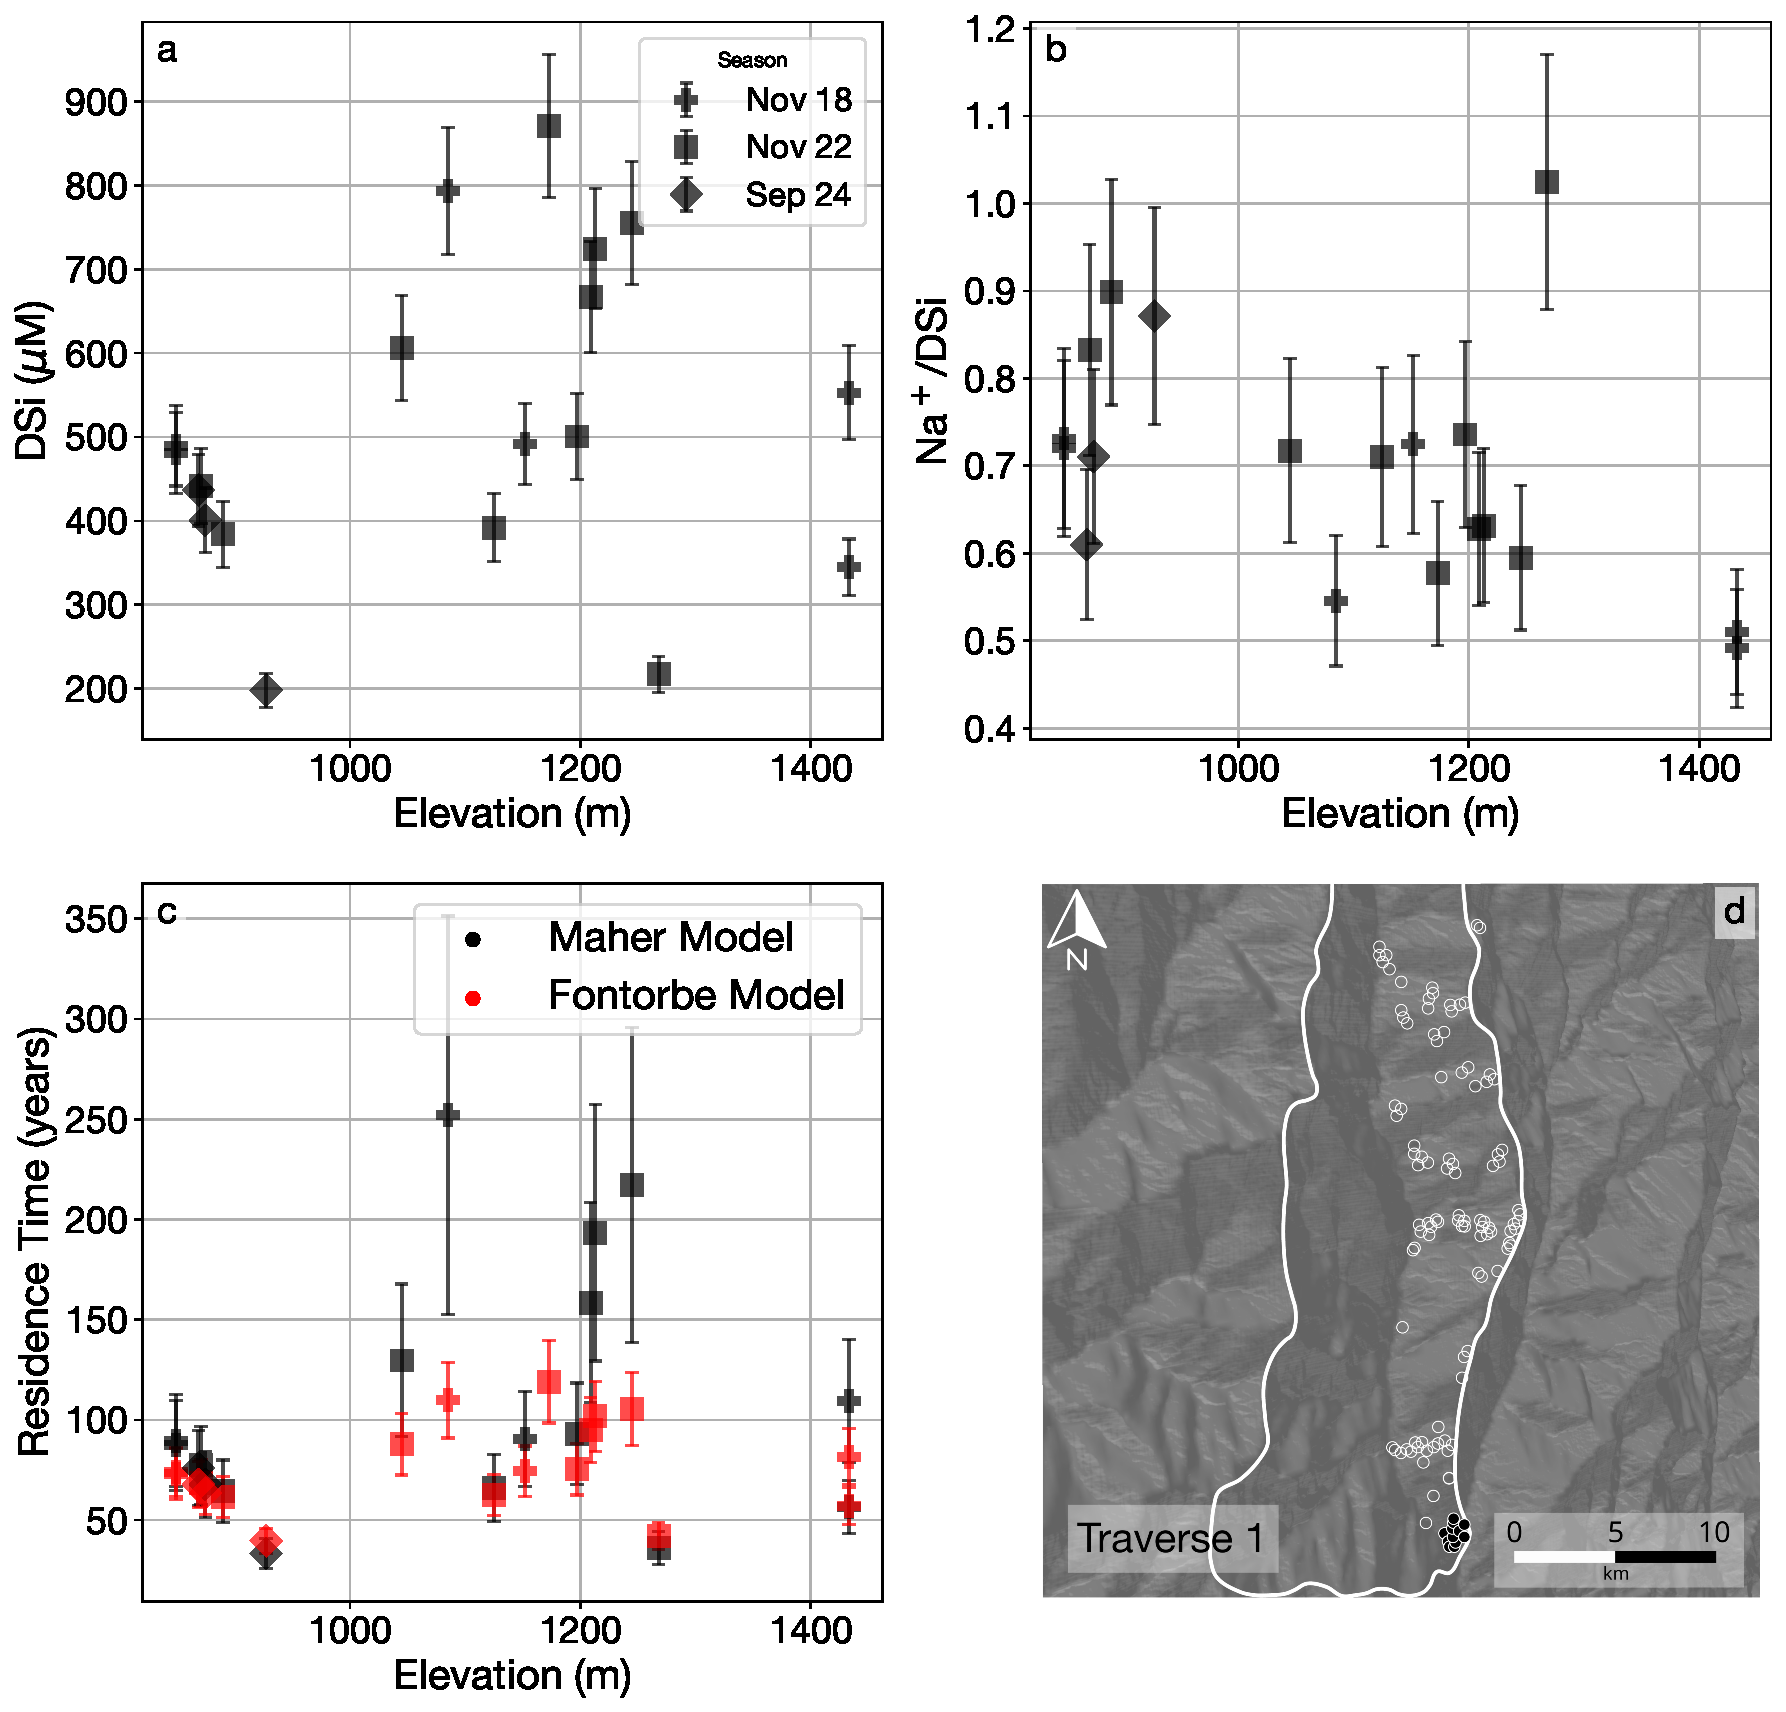
\includegraphics[width=\textwidth]{Traverse_1_summary.pdf}
    \caption{Traverse 1 - Variations in Spatial Chemistry}
    \label{fig:spatial_changes_spring1}
\end{figure}

\FloatBarrier

Concentration of dissolved silicon (DSi) in the springs sampled in Traverse 1 is at a maximum for the whole catchment. There is no clear trend of increasing DSi concentration or Na/Si with decreasing elevation. The Fontorbe model predicts a peak of $\approx$ 100 years, while the Maher model predicts a much higher residence time of $\approx$ 600 years. 




\newpage

\subsection{Traverse 2}

\begin{figure}[h]
    \centering
        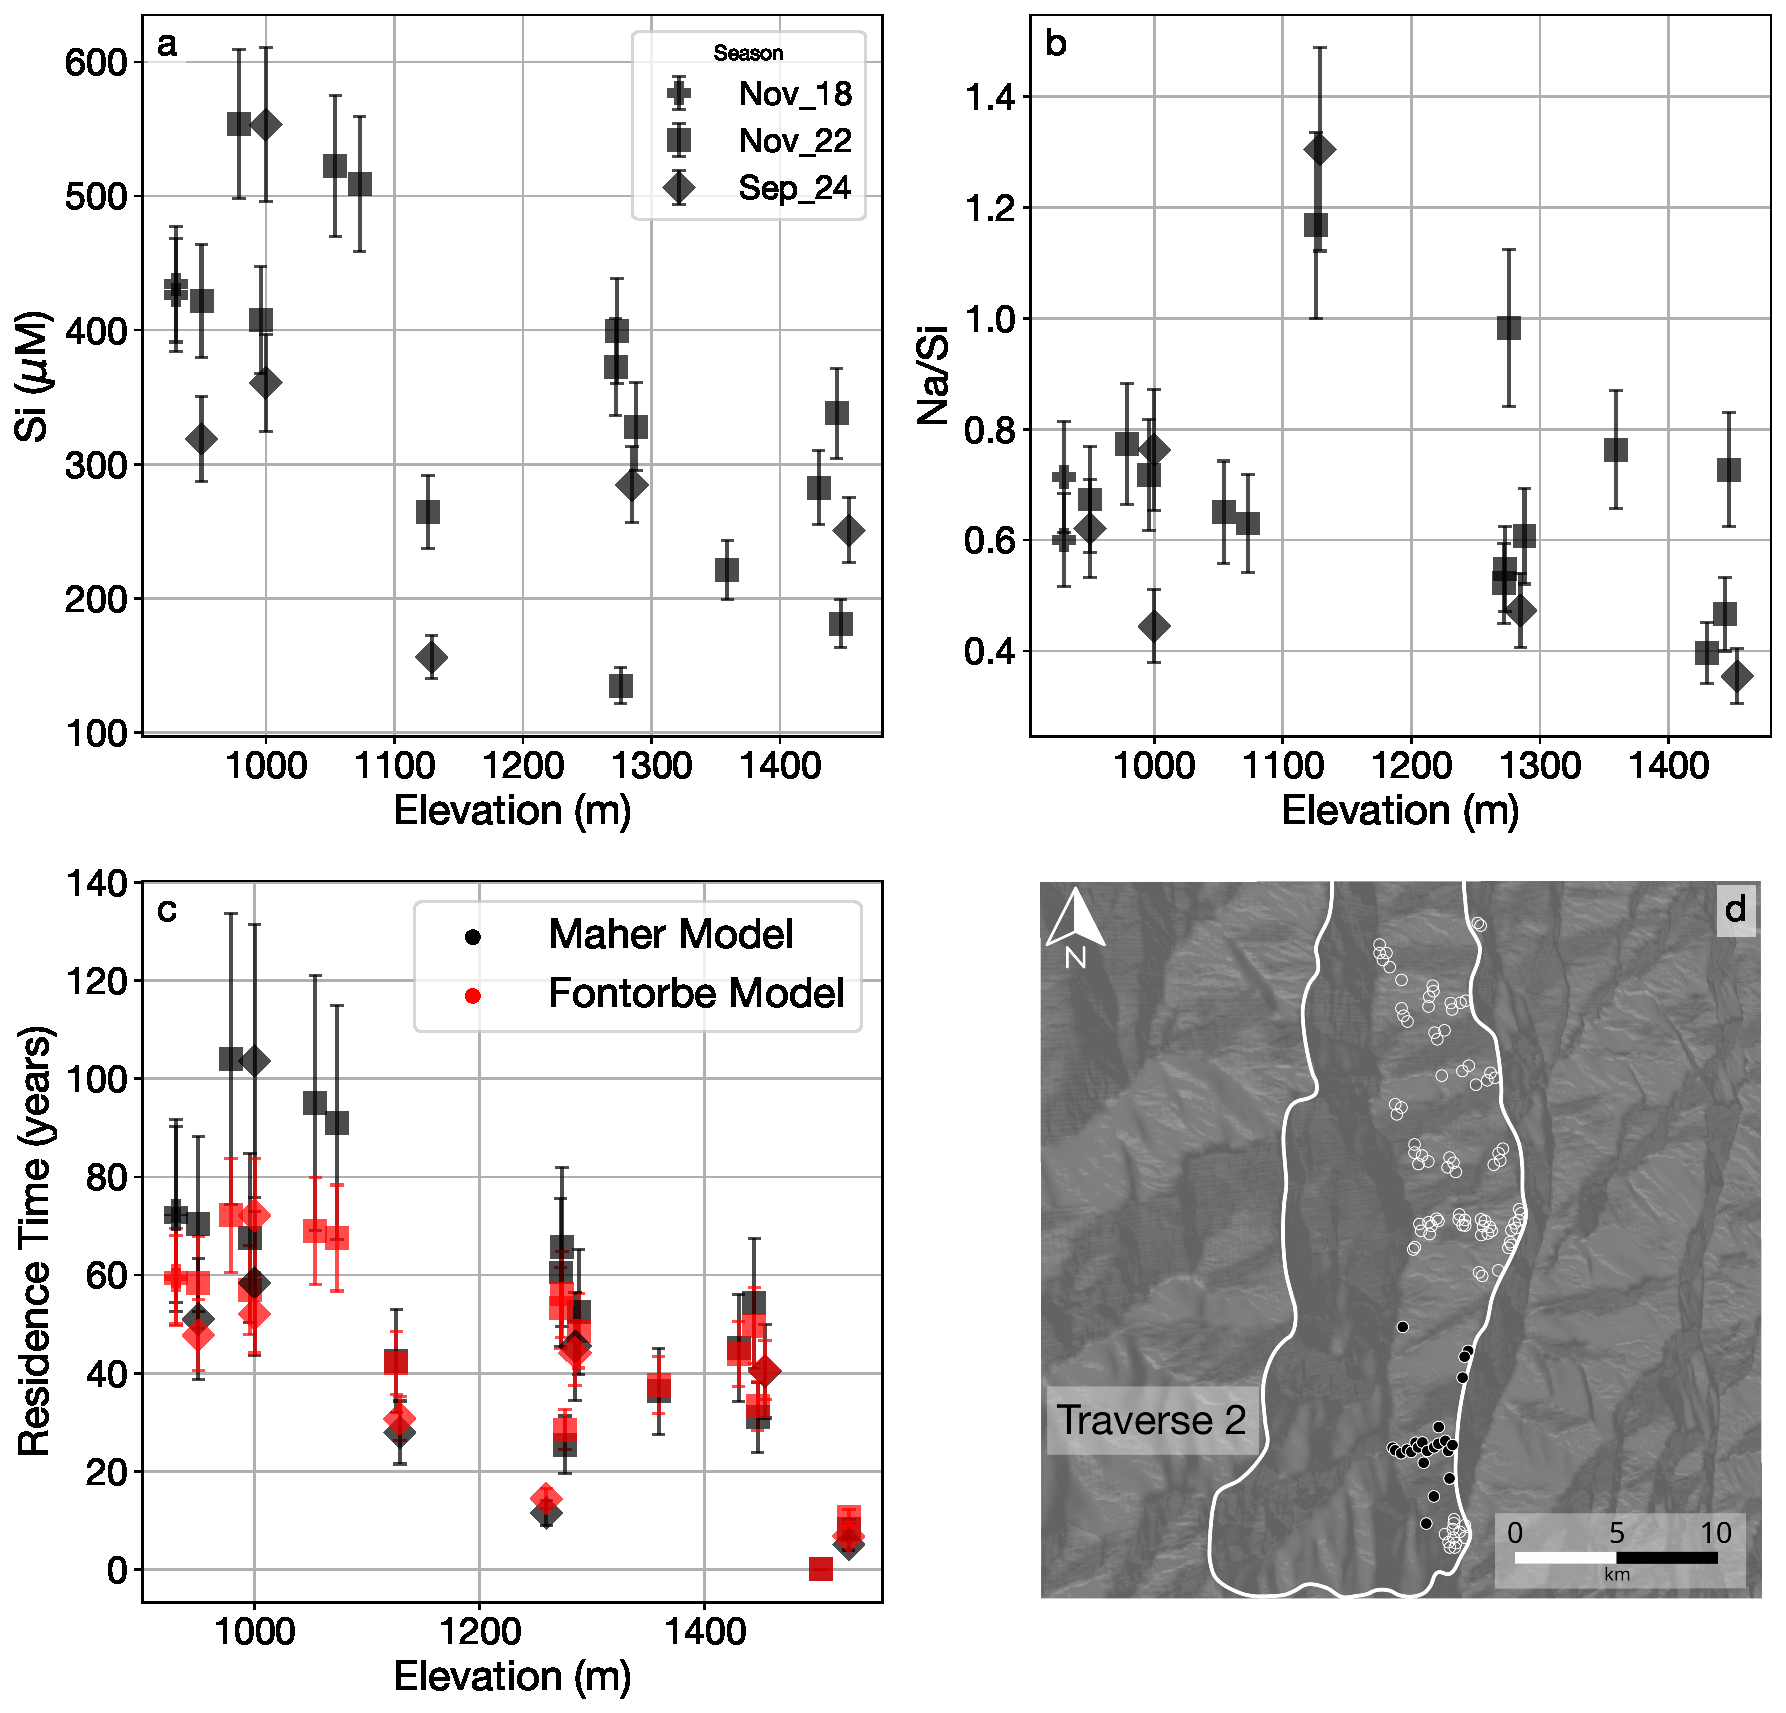
\includegraphics[width=\textwidth]{Traverse_2_summary.pdf}
    \caption{Traverse 2 - Variations in Spatial Chemistry}
    \label{fig:spatial_changes_spring2}
\end{figure}

\FloatBarrier

Dissolved silicon concentration shows a clear increase in concentration with decreasing elevation. There is no resolvable trend with Na/Si and elevation, nor with different seasons when it was collected. Residence times are generally lower than those in Traverse 1. The Fontorbe model predicts generally older times than the Maher model at higher elevations, and younger times at lower elevations. 




\newpage

\subsection{Traverse 3}

\begin{figure}[h]
    \centering
        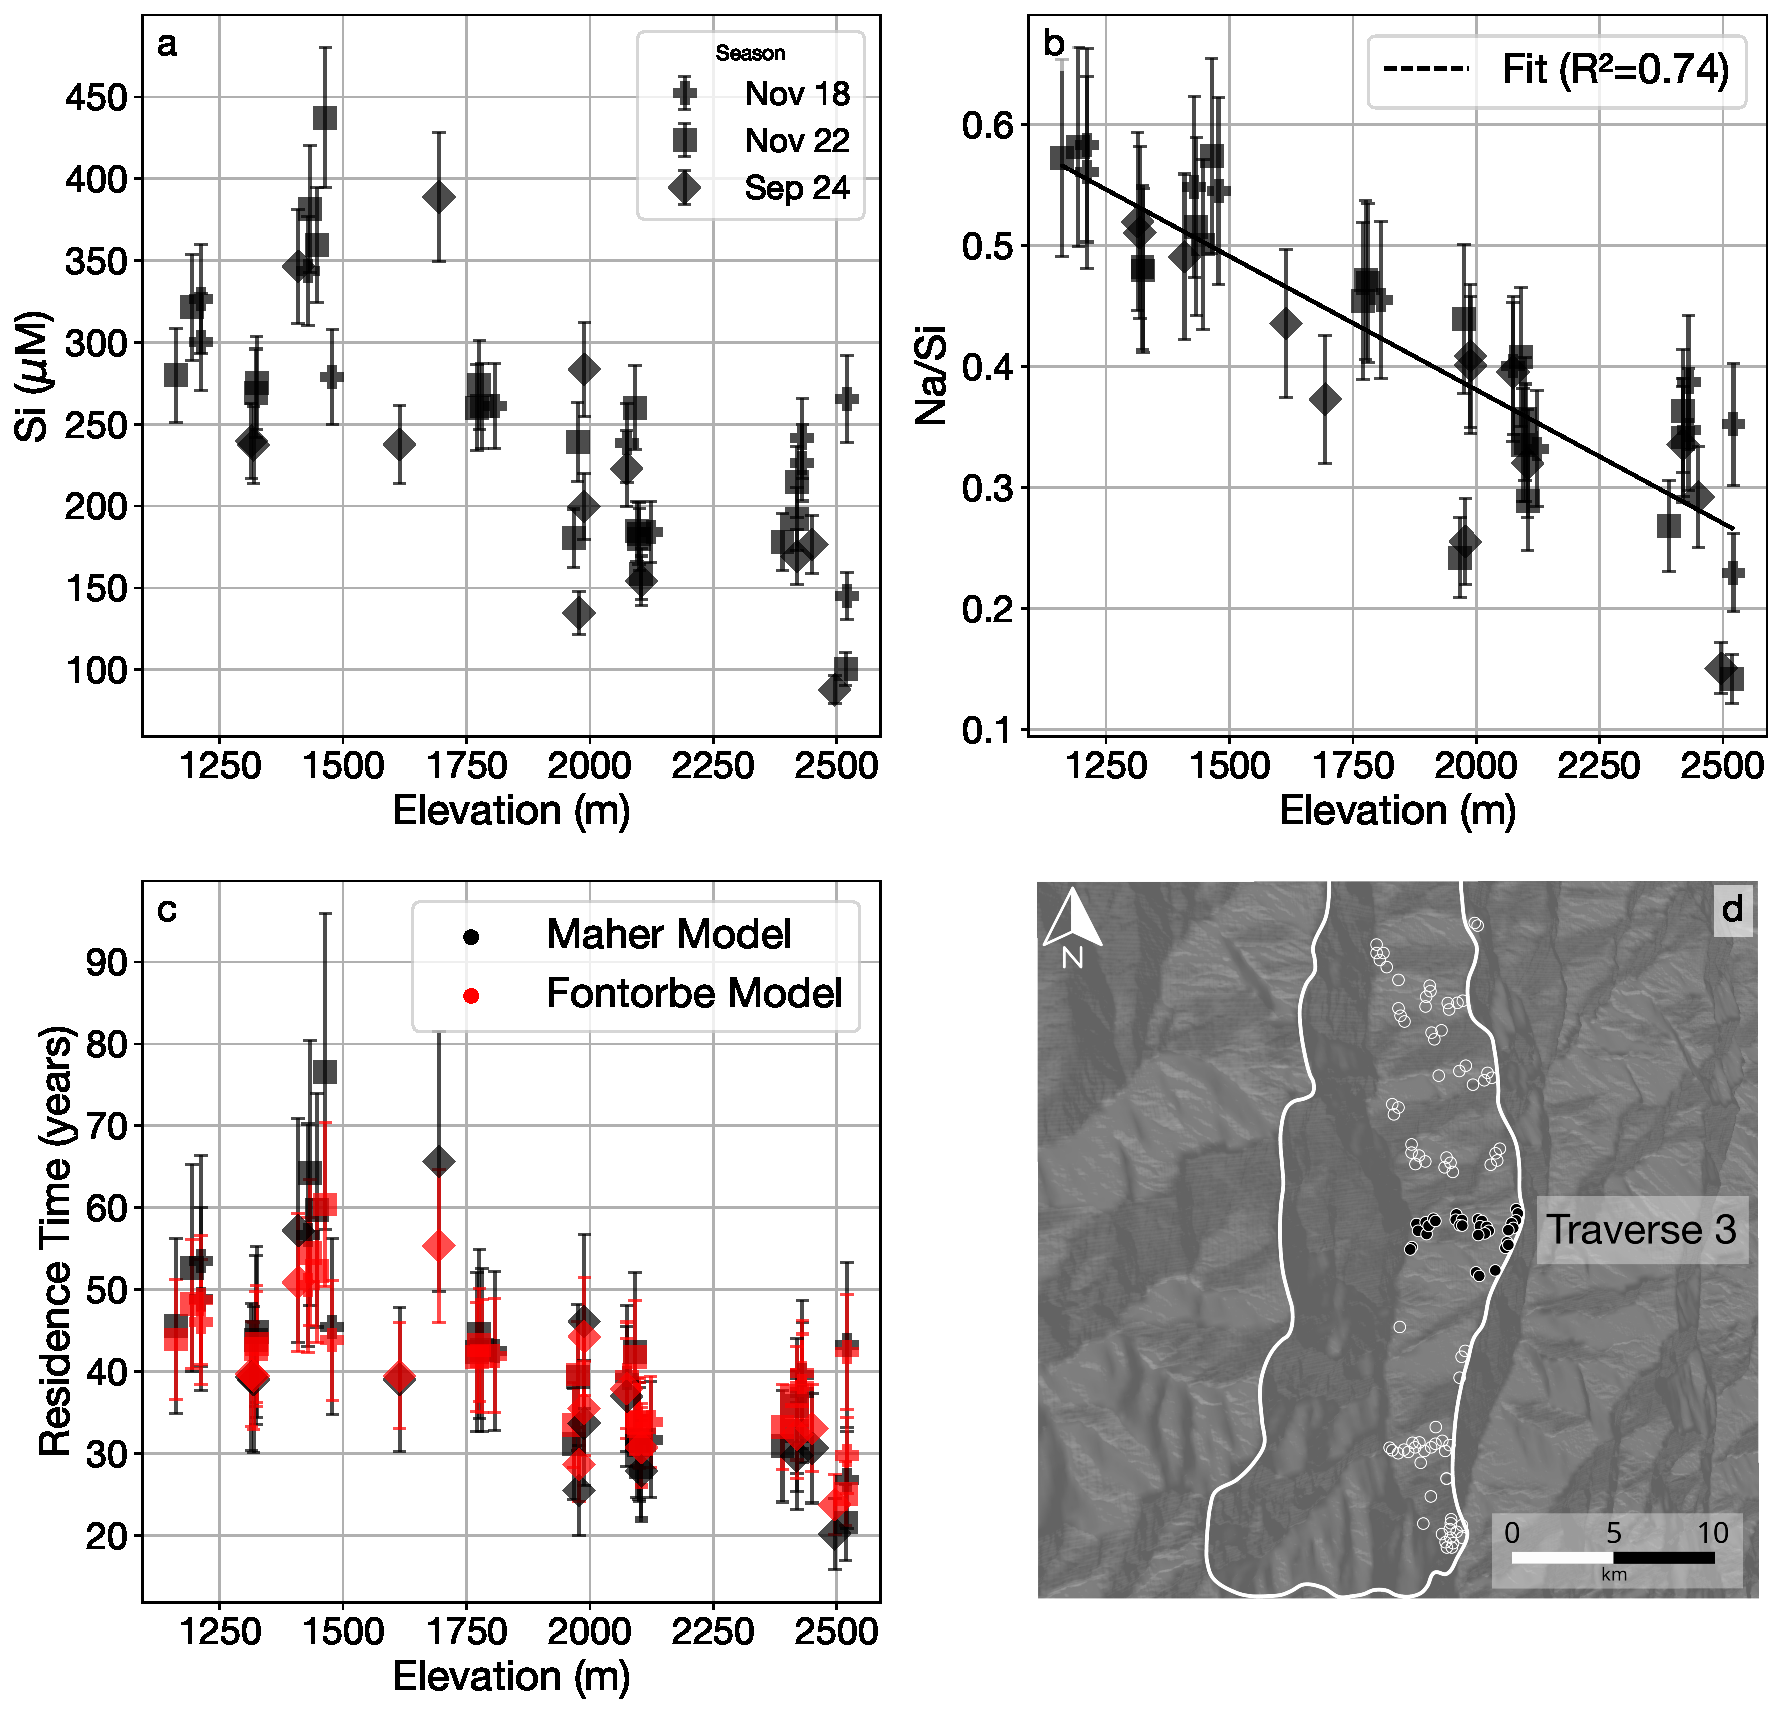
\includegraphics[width=\textwidth]{Traverse_3_summary.pdf}
    \caption{Traverse 3 - Variations in Spatial Chemistry}
    \label{fig:spatial_changes_spring3}
\end{figure}

\FloatBarrier

Dissolved silicon concentration increases with decreasing elevation in Traverse 3. There is a potential dip at the lowermost elevation sampled. Na/Si increases with decreasing elevation, consistent between different sampling seasons. Estimated residence times increase as elevation decreases, peaking at $\approx$ 50 years for the Maher model. This peak occurs at the same elevation as the highest DSi concentration.


\newpage

\subsection{Traverse 4}

\begin{figure}[h]
    \centering
        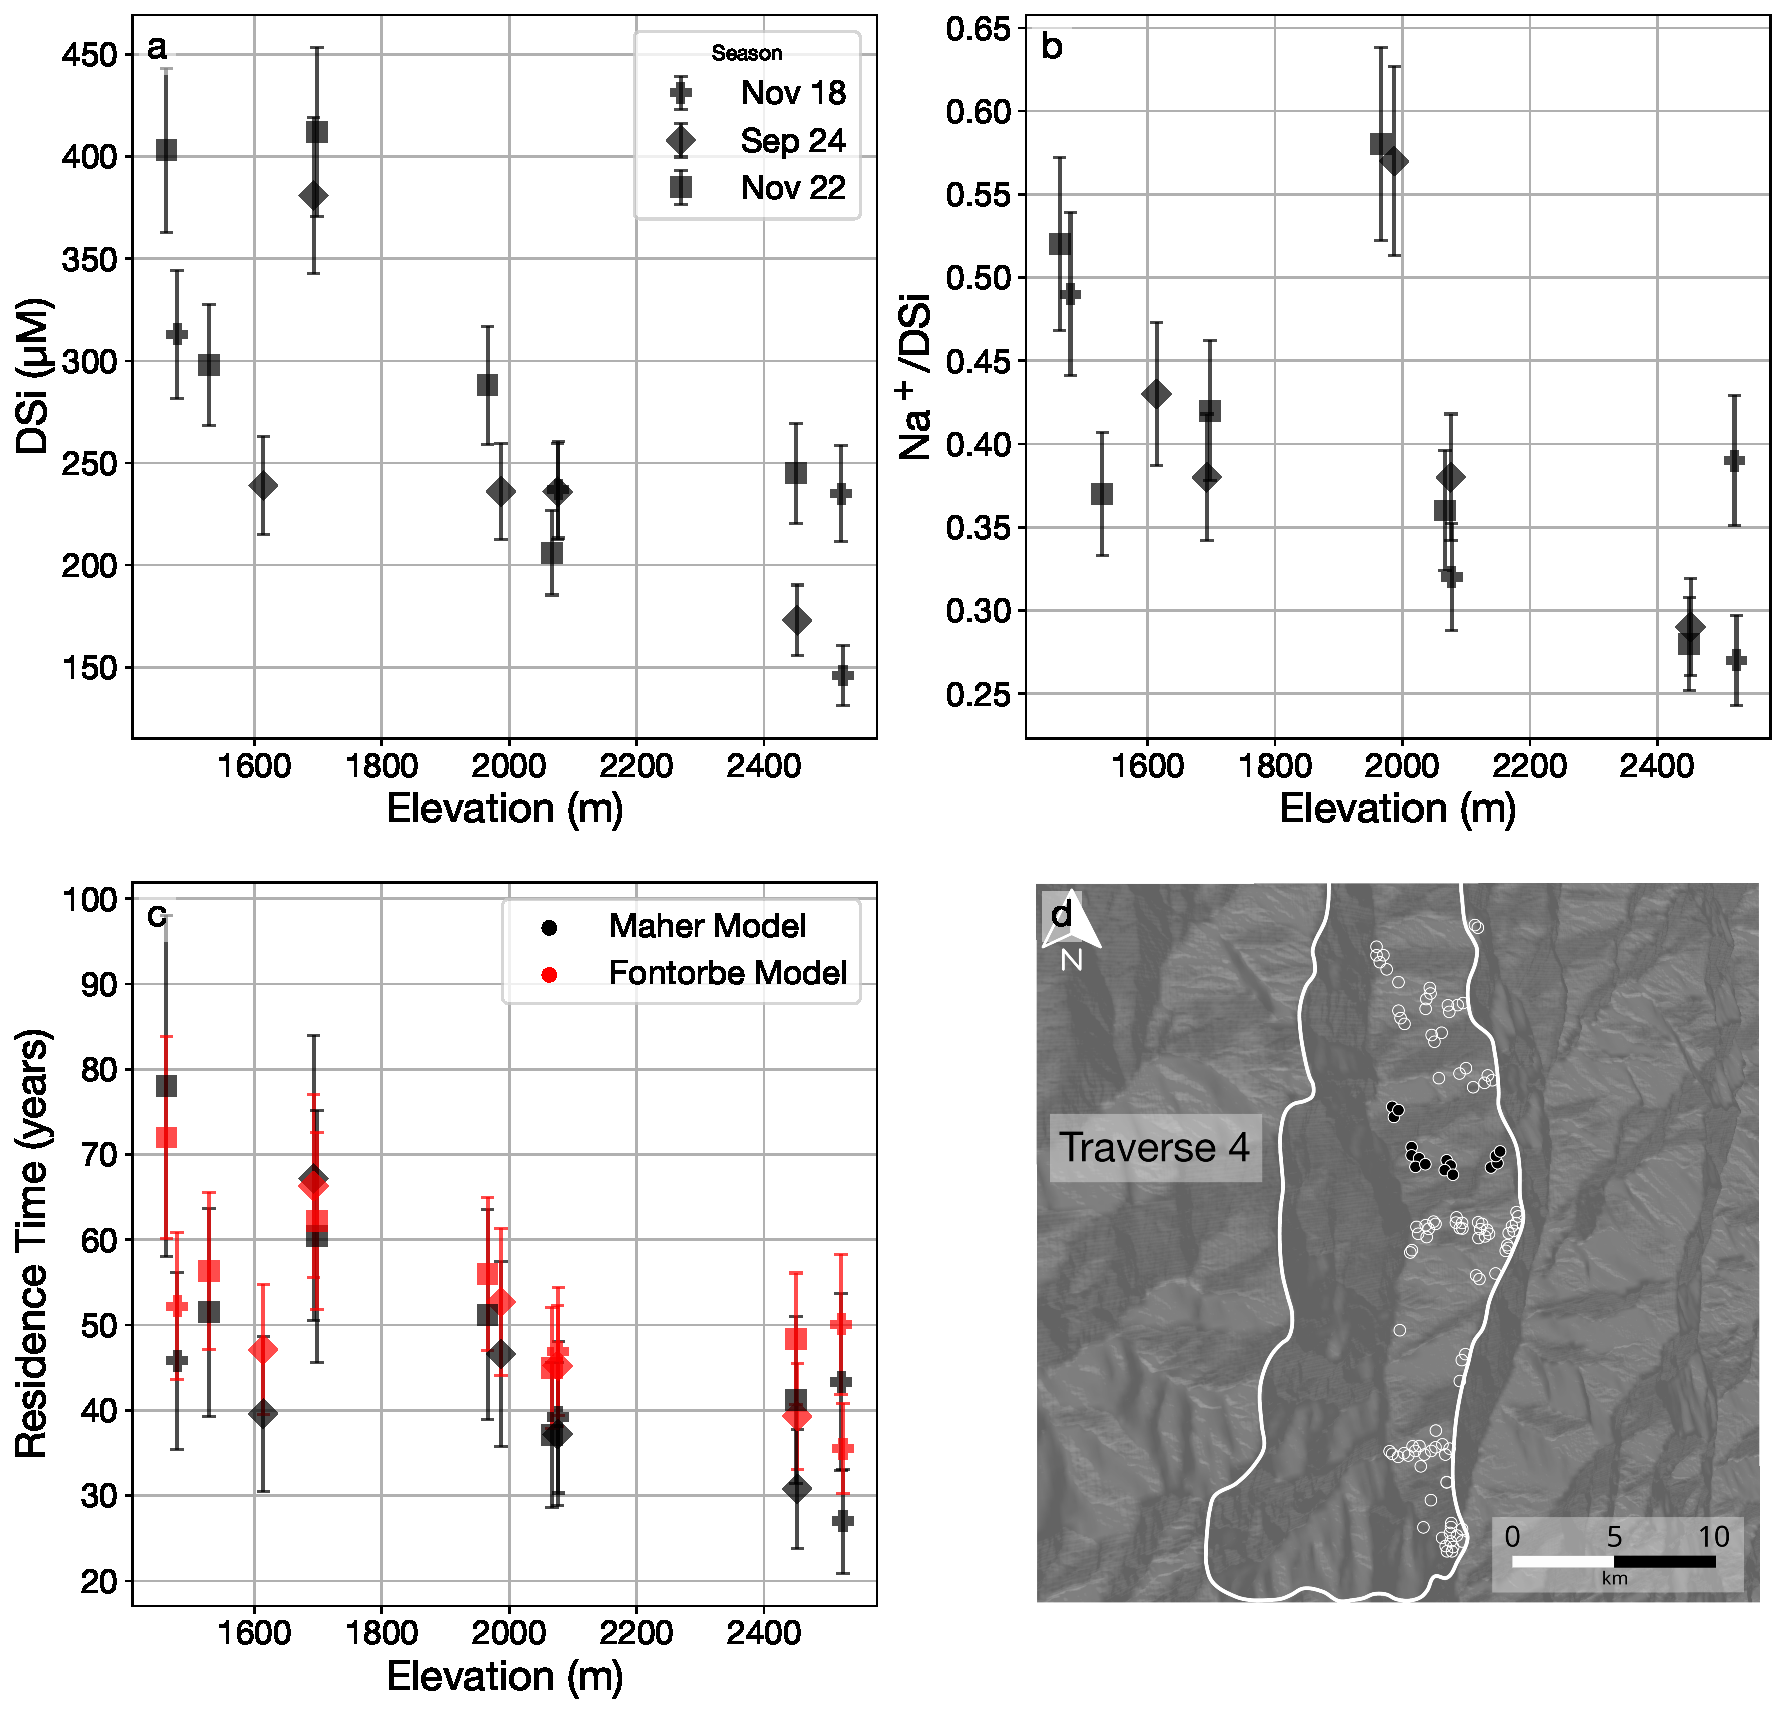
\includegraphics[width=\textwidth]{Traverse_4_summary.pdf}
    \caption{Traverse 4 - Variations in Spatial Chemistry}
    \label{fig:spatial_changes_spring4}
\end{figure}

\FloatBarrier

Traverse 4 is undersampled compared to the other traverses. Given the small sample set, any apparent trend is less to be reflective of the true chemistry. Nevertheless, DSi increases with decreasing elevation as seen in some of the previous traverses. There is no discernable trend with Na/Si. Residence times also increase with decreasing elevation, with the Maher model predicting younger times at the highest elevations, and older times at the lowest elevations. The highest residence times predicted are $\approx$ 35 years.


\newpage

\subsection{Traverse 5}

\begin{figure}[h]
    \centering
        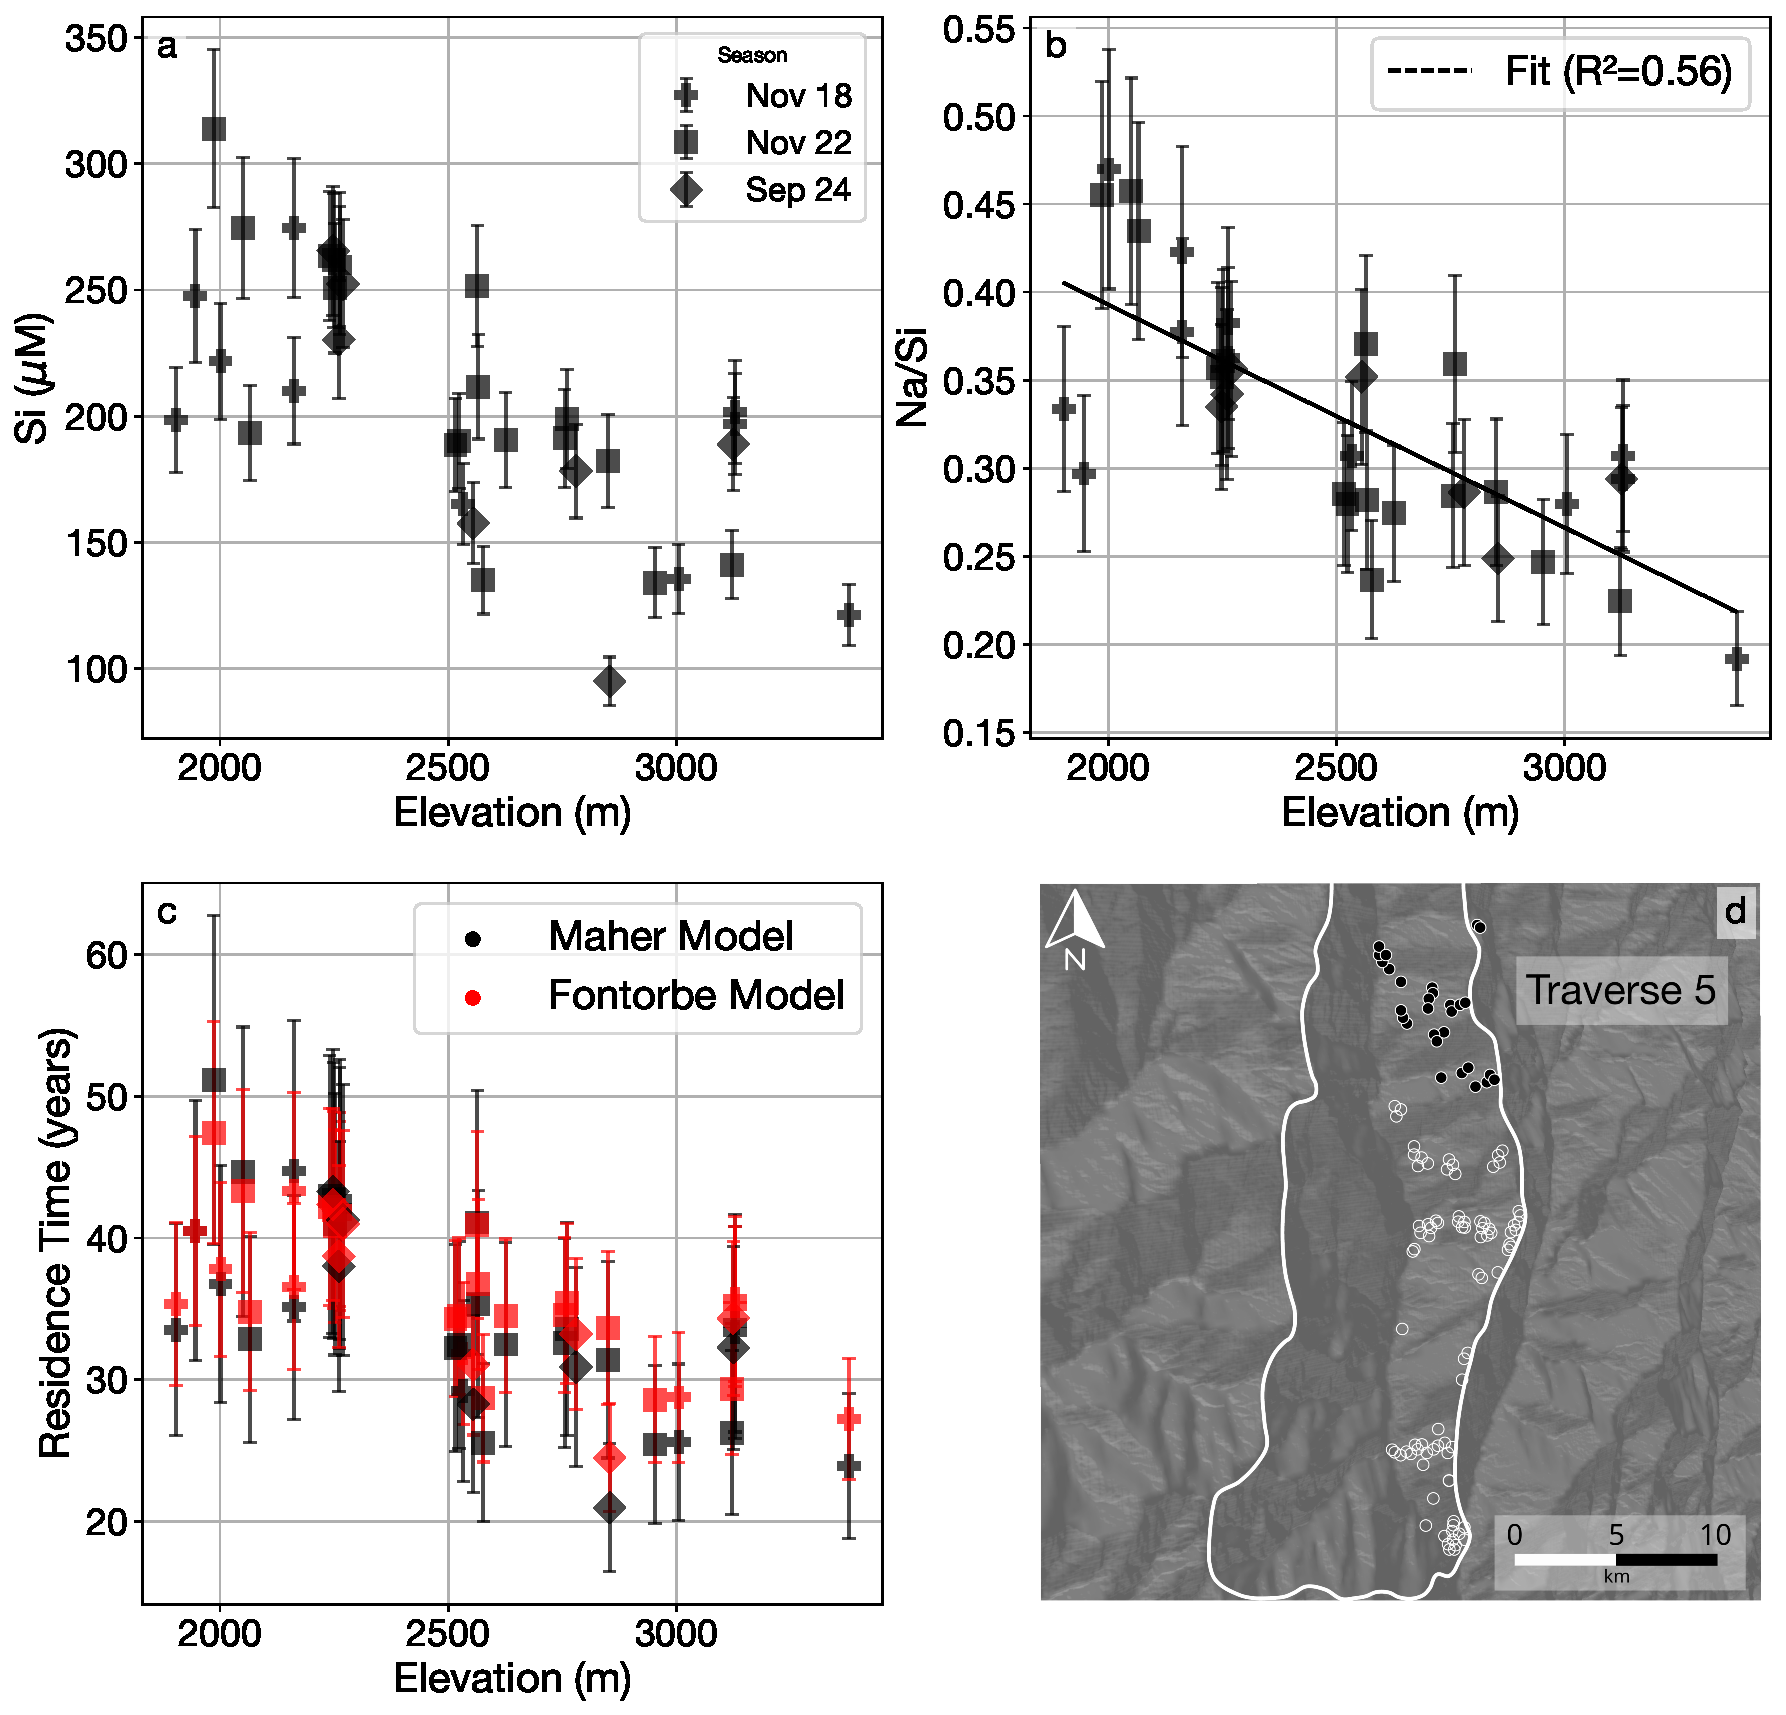
\includegraphics[width=\textwidth]{Traverse_5_summary.pdf}
    \caption{Traverse 5 - Variations in Spatial Chemistry}
    \label{fig:spatial_changes_spring5}
\end{figure}

\FloatBarrier

Traverse 5 is highly sampled and sits at the highest elevation of the whole catchment. DSi concentration increases with decreasing elevation but there is scatter in the data. Na/Si similarly shows a trend of increasing ratio with decreasing elevation, and it is replicated between different seasons, with considerable scatter. Residence times are the lowest predicted in the catchments.


\subsection{Time Series Trends}

Concentrations of dissolved silicon in several springs in the catchment show a consistent decrease in concentration with the onset of the monsoon. Concentrations are high in April, decrease to a minimum in September, then slowly increase back to April levels through October and November. Decrease in concentration is likely a sign of dilution from increased precipitation during the monsoon. Such a trend is also present in a time series of a spring in Traverse 3. The average April-September decrease is small compared to the average dissolved silicon concentration of the rain.


\begin{figure}[h]
    \centering
    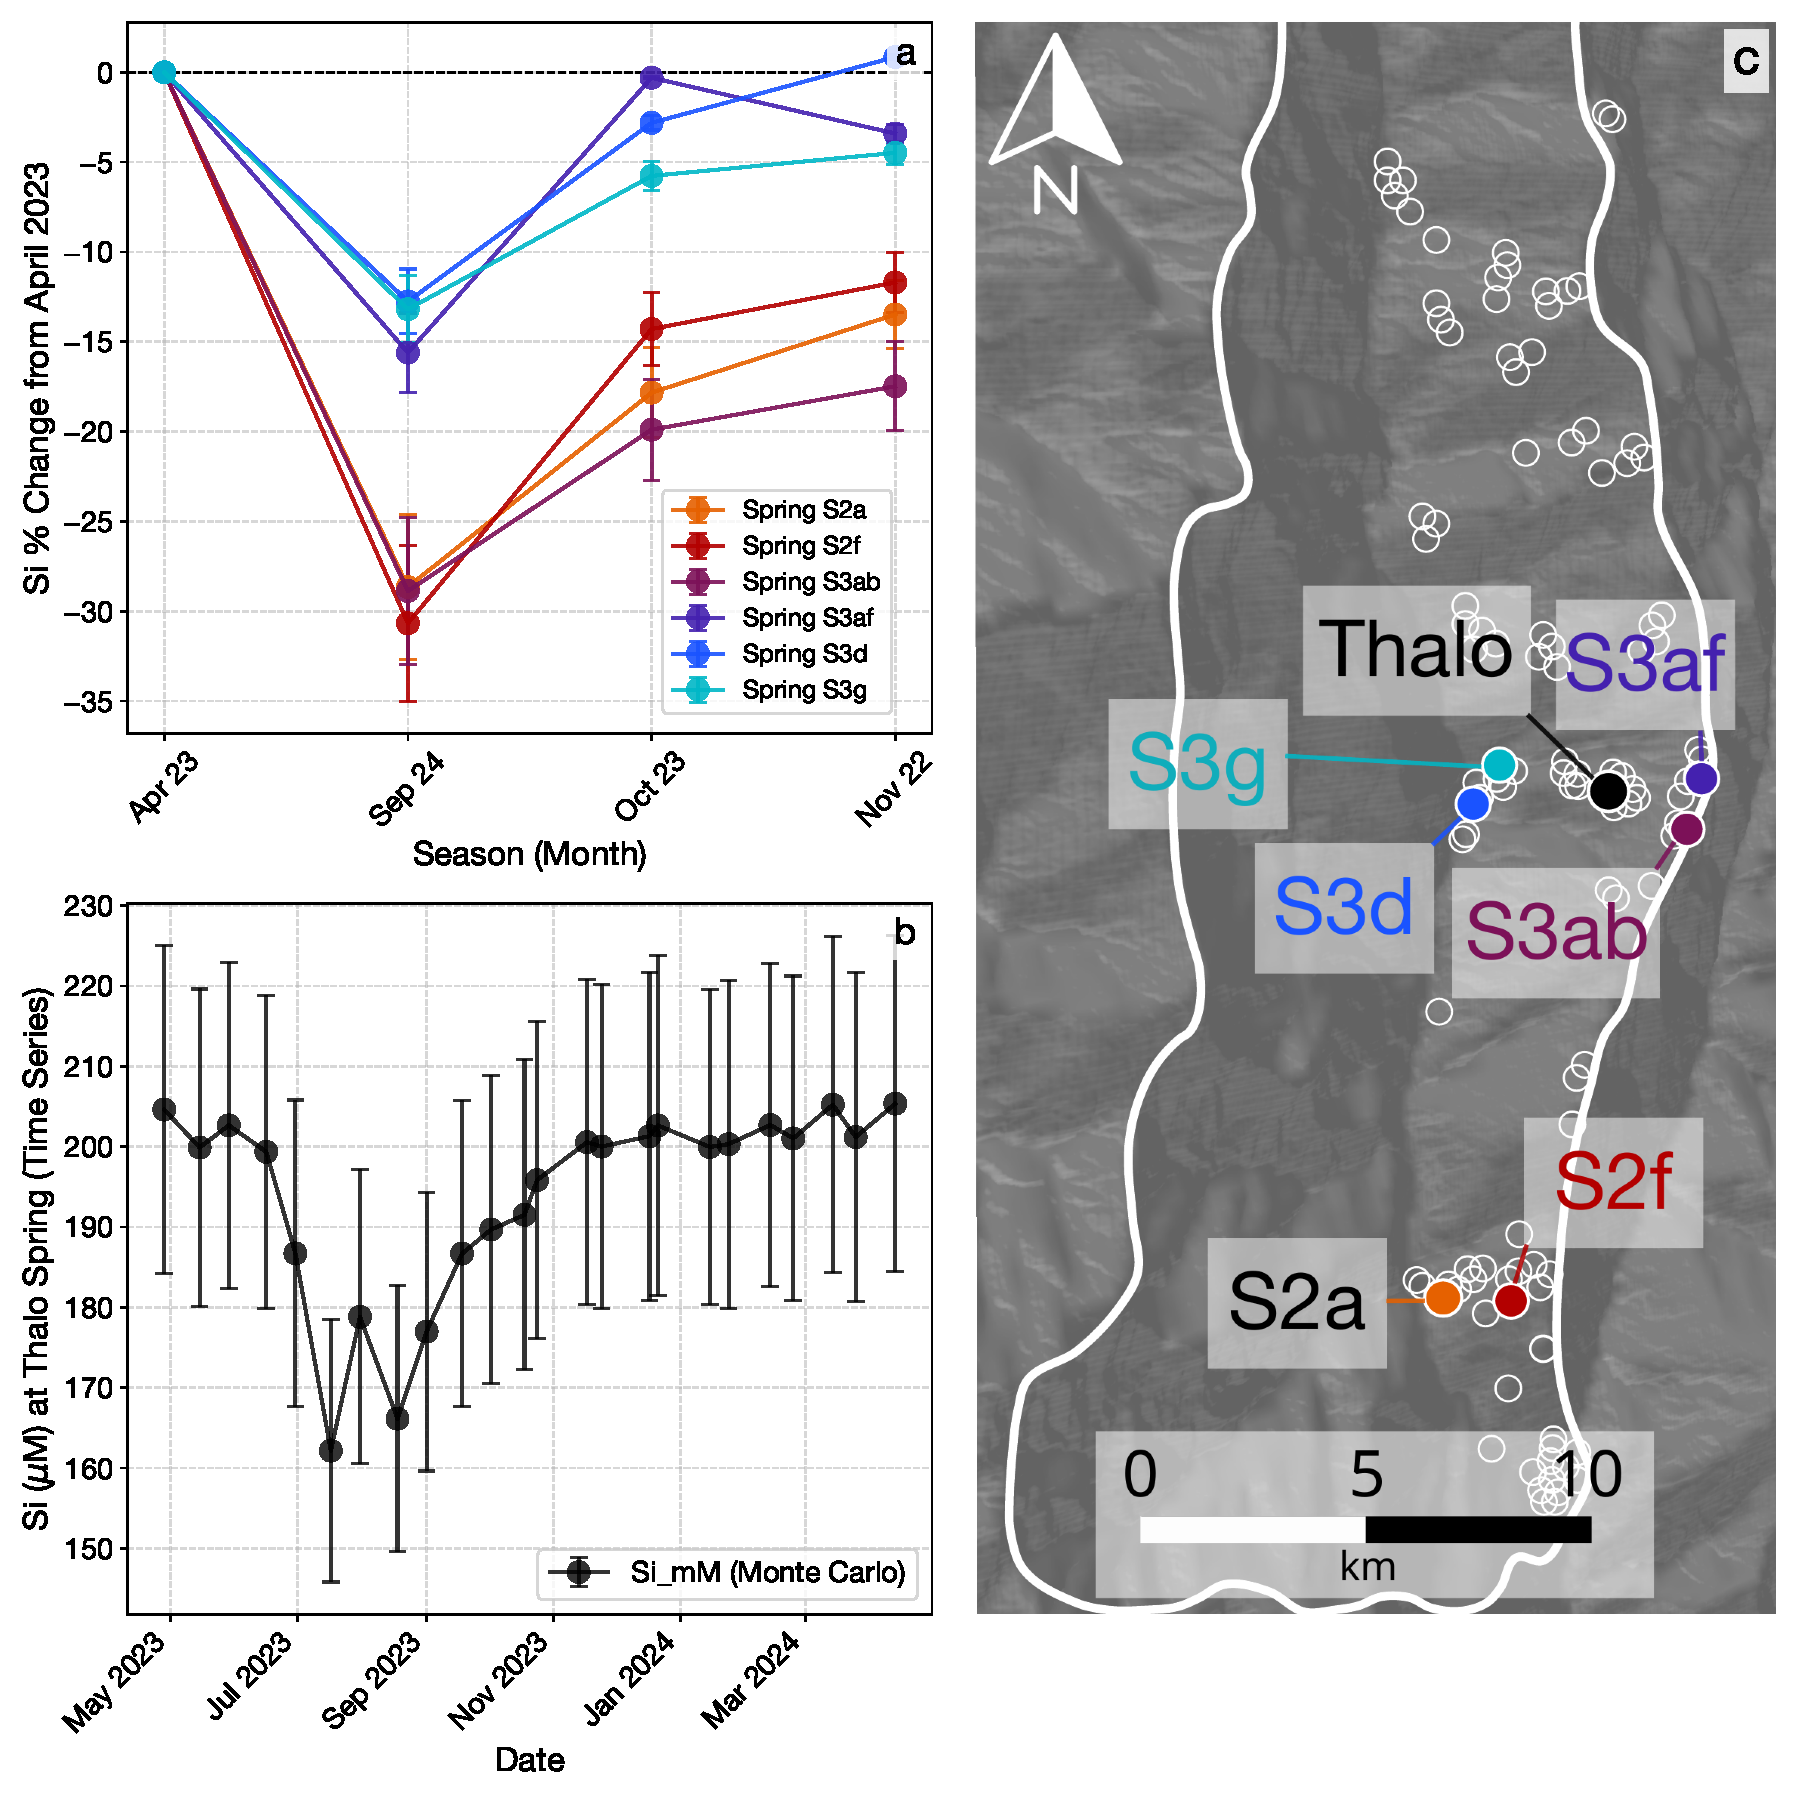
\includegraphics[width=0.9\textwidth]{Combined_Si_mM_Plots_with_Schematic.pdf}
    \caption{Seasonal changes in spring concentration indicating monsoonal precipitation influence.; Time series of spring concentration changes over time.}
    \label{fig:time_series_changes}
\end{figure}

\FloatBarrier

















% \subsection{Strontium Isotope Values of Springs and Rain}



% \begin{landscape} % Start landscape mode

%     \scriptsize  % Reduce font size for better fit

%     \noindent % Avoid indentation
%     \begin{minipage}{0.48\linewidth} % First half of the landscape page

%         \begin{longtable}{l r r l r r}
%             \caption{Strontium isotope values (Part 1)} \label{tab:sr87_sr86_data1} \\
%             \hline
%             \textbf{Sample ID} & \textbf{Elevation (m)} & \textbf{pH} & \boldmath{$^{87}$Sr/$^{86}$Sr} (\textbf{2SD} $\cdot$10$^{\text{6}}$)} & \textbf{Sr ($\mu$M)} & \textbf{Cl ($\mu$M)} \\
%             \hline
%             \endfirsthead

%             \multicolumn{6}{c}{\textbf{(Continued from previous page)}} \\
%             \hline
%             \textbf{Sample ID} & \textbf{Elevation (m)} & \textbf{pH} & \boldmath{$^{87}$Sr/$^{86}$Sr} (\textbf{2SD} $\cdot$10$^{\text{6}}$)} & \textbf{Sr ($\mu$M)} & \textbf{Cl ($\mu$M)} \\
%             \hline
%             \endhead

%             \hline
%             \multicolumn{6}{r}{\textit{Continued on next column}} \\
%             \endfoot

%             \hline
%             \endlastfoot


%             \multicolumn{6}{c}{\textbf{Rain}} \\

%             NEP24-039 & 840 & 6.79 & 0.73906 \hfill (24) & 0.13 & 28.09 \\
%             NEP24-043 & 1351 & 5.82 & 0.71442 \hfill (46) & 0.01 & 3.55 \\
%             NEP24-044 & 1952 & 6.05 & 0.71352 \hfill (127) & 0.01 & 1.89 \\
%             NEP24-045 & 2644 & 5.00 & 0.71292 \hfill (73) & 0.01 & 3.21 \\
%             NEP24-046 & 2110 & 6.02 & 0.70904 \hfill (100) & 0.02 & 2.86 \\
%             NEP24-047 & 2644 & 5.74 & 0.71194 \hfill (237) & 0.01 & 0.55 \\
%             NEP24-048 & 2644 & 5.61 & 0.71182 \hfill (189) & 0.01 & 3.65 \\
%             \hline

%             \multicolumn{6}{c}{\textbf{Traverse 1}} \\
%             NEP22-1 & 871 & 7.08 & 0.74101 \hfill (29) & 0.34 & 81.09 \\
%             NEP22-2 & 890 & 7.75 & 0.74115 \hfill (22) & 0.35 & 92.95 \\
%             NEP22-80 & 1045 & 7.71 & 0.75192 \hfill (33) & 0.26 & 6.43 \\
%             NEP22-81 & 1209 & 7.89 & 0.75506 \hfill (27) & 0.21 & 10.64 \\
%             NEP22-82 & 1213 & 7.04 & 0.75517 \hfill (23) & 0.31 & 13.10 \\
%             NEP22-83 & 1245 & 6.24 & 0.75154 \hfill (27) & 0.31 & 4.31 \\
%             NEP22-84 & 1173 & 7.86 & 0.74969 \hfill (61) & 0.28 & 3.17 \\
%             NEP22-85 & 1197 & 7.56 & 0.75394 \hfill (32) & 0.16 & 2.38 \\
%             NEP22-86 & 1125 & 8.27 & 0.75957 \hfill (35) & 0.07 & 54.46 \\
%             NEP22-87 & 1268 & 6.26 & 0.74341 \hfill (25) & 0.78 & 223.01 \\
%             \hline
            
%             \multicolumn{6}{c}{\textbf{Traverse 2}} \\

%             NEP22-61 & 1528 & 5.32 & 0.74691 \hfill (62) & 0.29 & 349.74 \\
%             NEP22-62 & 1503 & 6.41 & 0.73943 \hfill (25) & 0.06 & 362.10 \\
%             NEP22-63 & 1447 & 6.73 & 0.74943 \hfill (37) & 0.47 & 152.05 \\
%             NEP22-64 & 1444 & 6.53 & 0.74872 \hfill (25) & 0.33 & 101.99 \\
%             NEP22-65 & 1430 & 6.51 & 0.74886 \hfill (30) & 0.17 & 58.79 \\
%             NEP22-66 & 1359 & 7.35 & 0.74629 \hfill (30) & 0.03 & 126.02 \\
%             NEP22-67 & 1126 & 6.83 & 0.74510 \hfill (41) & 0.48 & 235.79 \\
%             NEP22-68 & 1288 & 5.42 & 0.75696 \hfill (23) & 0.29 & 112.71 \\
%             NEP22-70 & 950 & 7.54 & 0.73128 \hfill (37) & 1.18 & 60.86 \\
%             NEP22-71 & 996 & 7.99 & 0.74253 \hfill (42) & 0.31 & 125.59 \\
%             NEP22-73 & 979 & 6.73 & 0.73191 \hfill (19) & 0.86 & 41.91 \\
%             NEP22-75 & 1054 & 6.53 & 0.73921 \hfill (71) & 0.46 & 117.33 \\
%             NEP22-76 & 1073 & 6.82 & 0.73701 \hfill (21) & 0.43 & 111.78 \\
%             NEP22-78 & 1272 & 6.74 & 0.74584 \hfill (36) & 0.17 & 40.32 \\
%             NEP22-79 & 1276 & 5.67 & 0.74752 \hfill (56) & 0.29 & 305.63 \\
%             \hline

%         \end{longtable}

%     \end{minipage} % End first column

%     \hfill % Add space between tables

%     \begin{minipage}{0.48\linewidth} % Second half of the landscape page

%         \begin{longtable}{l r r l r r}
%             \caption{Strontium isotope values (Part 2)} \label{tab:sr87_sr86_data2} \\
%             \hline
%             \textbf{Sample ID} & \textbf{Elevation (m)} & \textbf{pH} & \boldmath{$^{87}$Sr/$^{86}$Sr} (\textbf{2SD} $\cdot$10$^{\text{6}}$)} & \textbf{Sr ($\mu$M)} & \textbf{Cl ($\mu$M)} \\
%             \hline
%             \endfirsthead

%             \multicolumn{6}{c}{\textbf{(Continued from previous page)}} \\
%             \hline
%             \textbf{Sample ID} & \textbf{Elevation (m)} & \textbf{pH} & \boldmath{$^{87}$Sr/$^{86}$Sr} (\textbf{2SD} $\cdot$10$^{\text{6}}$)} & \textbf{Sr ($\mu$M)} & \textbf{Cl ($\mu$M)} \\
%             \hline
%             \endhead

%             \hline
%             \multicolumn{6}{r}{\textit{Continued on next page}} \\
%             \endfoot

%             \hline
%             \endlastfoot

%             \multicolumn{6}{c}{\textbf{Traverse 3}} \\

%             NEP22-10 & 2419 & 6.48 & 0.73918 \hfill (60) & 0.20 & 17.13 \\
%             NEP22-11 & 2419 & 6.59 & 0.73819 \hfill (20) & 0.22 & 15.76 \\
%             NEP22-12 & 2390 & 6.77 & 0.73162 \hfill (27) & 0.16 & 2.89 \\
%             NEP22-13 & 2099 & 6.76 & 0.73614 \hfill (54) & 0.25 & 9.03 \\
%             NEP22-15 & 1975 & 7.29 & 0.73841 \hfill (14) & 0.23 & 4.98 \\
%             NEP22-16 & 1967 & 7.14 & 0.73370 \hfill (22) & 0.15 & 1.05 \\
%             NEP22-17 & 2100 & 6.90 & 0.73584 \hfill (26) & 0.21 & 11.74 \\
%             NEP22-18 & 2091 & 6.98 & 0.73281 \hfill (19) & 0.38 & 8.66 \\
%             NEP22-19 & 2095 & 6.07 & 0.73594 \hfill (28) & 0.25 & 9.44 \\
%             NEP22-20 & 2104 & 7.14 & 0.73241 \hfill (34) & 0.11 & 6.87 \\
%             NEP22-42 & 1325 & 6.24 & 0.73680 \hfill (62) & 0.31 & 27.25 \\
%             NEP22-45 & 1194 & 7.57 & 0.73763 \hfill (22) & 0.32 & 23.90 \\
%             NEP22-53 & 1776 & 6.33 & 0.73720 \hfill (39) & 0.40 & 19.70 \\
%             NEP22-54 & 1781 & 6.19 & 0.73831 \hfill (18) & 0.36 & 20.39 \\
%             NEP22-55 & 1771 & 6.69 & 0.73824 \hfill (19) & 0.36 & 19.57 \\
%             NEP22-56 & 1433 & 6.86 & 0.74129 \hfill (26) & 0.42 & 23.24 \\
%             NEP22-57 & 1464 & 6.85 & 0.73240 \hfill (37) & 0.69 & 46.41 \\
%             NEP22-58 & 1447 & 7.34 & 0.73871 \hfill (19) & 0.36 & 7.57 \\
%             NEP22-59 & 1324 & 7.48 & 0.73780 \hfill (73) & 0.32 & 14.91 \\
%             NEP22-60 & 1161 & 7.04 & 0.73121 \hfill (24) & 0.38 & 22.66 \\
%             NEP24-010 & 1314 & 6.45 & 0.73689 \hfill (94) & 0.31 & 21.65 \\
%             NEP24-011 & 1319 & 7.07 & 0.73782 \hfill (29) & 0.33 & 10.92 \\
%             NEP24-014 & 2496 & 6.58 & 0.73508 \hfill (0) & 0.03 & 1.84 \\
%             NEP24-015 & 2104 & 6.10 & 0.73644 \hfill (47) & 0.20 & 7.38 \\
%             NEP24-016 & 1978 & 7.05 & 0.73360 \hfill (20) & 0.16 & 0.39 \\
%             \hline
%             \multicolumn{6}{c}{\textbf{Traverse 4}} \\

%             NEP22-46 & 2555 & 7.05 & 0.74922 \hfill (56) & 0.16 & 3.37 \\
%             NEP22-47 & 2451 & 6.65 & 0.73661 \hfill (36) & 0.19 & 7.65 \\
%             NEP22-48 & 2067 & 6.63 & 0.74727 \hfill (28) & 0.22 & 2.64 \\
%             NEP22-49 & 1968 & 6.88 & 0.73730 \hfill (28) & 0.44 & 5.12 \\
%             NEP22-50 & 1698 & 6.69 & 0.73508 \hfill (39) & 0.62 & 21.22 \\
%             NEP22-52 & 1532 & 7.00 & 0.73828 \hfill (22) & 0.18 & 7.99 \\
%             \hline
%             \multicolumn{6}{c}{\textbf{Traverse 5}} \\

%             NEP22-22 & 2755 & 6.90 & 0.73006 \hfill (20) & 0.19 & 1.94 \\
%             NEP22-23 & 2516 & 6.17 & 0.73210 \hfill (26) & 0.13 & 1.19 \\
%             NEP22-24 & 2626 & 7.16 & 0.72989 \hfill (20) & 0.19 & 5.93 \\
%             NEP22-25 & 2566 & 7.24 & 0.72999 \hfill (44) & 0.24 & 4.23 \\
%             NEP22-26 & 2577 & 6.83 & 0.73230 \hfill (22) & 0.11 & 1.73 \\
%             NEP22-27 & 3122 & 7.00 & 0.73165 \hfill (35) & 0.09 & 1.53 \\
%             NEP22-28 & 2953 & 7.22 & 0.73238 \hfill (26) & 0.11 & 1.73 \\
%             NEP22-29 & 2850 & 7.24 & 0.73218 \hfill (22) & 0.15 & 1.71 \\
%             NEP22-30 & 2760 & 6.70 & 0.73243 \hfill (24) & 0.17 & 3.08 \\
%             NEP22-31 & 2564 & 6.90 & 0.73244 \hfill (25) & 0.28 & 1.96 \\
%             NEP22-32 & 2252 & 6.27 & 0.73227 \hfill (23) & 0.26 & 11.19 \\
%             NEP22-33 & 2249 & 7.51 & 0.73166 \hfill (20) & 0.26 & 13.14 \\
%             NEP22-34 & 2240 & 7.35 & 0.73155 \hfill (56) & 0.27 & 16.81 \\
%             NEP22-35 & 2066 & 7.55 & 0.73334 \hfill (19) & 0.16 & 2.78 \\
%             NEP22-36 & 1986 & 7.84 & 0.73205 \hfill (20) & 0.27 & 3.00 \\
%             NEP22-37 & 2050 & 7.72 & 0.73280 \hfill (44) & 0.22 & 2.33 \\
%             NEP22-39 & 2524 & 7.60 & 0.73116 \hfill (22) & 0.18 & 4.51 \\

%             \hline
%         \end{longtable}

%     \end{minipage} % End first column

% \end{landscape}


% \FloatBarrier


% Radiogenic strontium isotope analyses of springs show a wide variation between different traverses. Sr isotopes were also measured for the collected rain samples, and these range from 0.70904 to 0.73906. The lowest of these rain values is close to the reported value for seawater, which is 0.70917.  